\documentclass[a4paper, 11px]{article}

\usepackage[french]{babel}
\usepackage[utf8]{inputenc}
\usepackage{fancyhdr}
\usepackage{lastpage}
\usepackage{graphicx}
\usepackage{rotating}
\usepackage{textcomp}
\usepackage{xspace}
\usepackage[toc,page]{appendix}
\usepackage{array}
\usepackage{amssymb}
\usepackage{enumerate}
\usepackage{enumitem}
\usepackage{eso-pic}

% \usepackage{needspace}


%%%%%%
 
\usepackage{listings}

\lstset{
  morekeywords={},
  sensitive=f,
  morecomment=[l]--,
  morestring=[d]",
  showstringspaces=false,
  basicstyle=\small\ttfamily,
  keywordstyle=\bf\small,
  commentstyle=\itshape,
  stringstyle=\sf,
  extendedchars=true,
  columns=[c]fixed
}

% CI-DESSOUS: conversion des caractères accentués UTF-8 
% en caractères TeX dans les listings...
\lstset{
  literate=%
  {À}{{\`A}}1 {Â}{{\^A}}1 {Ç}{{\c{C}}}1%
  {à}{{\`a}}1 {â}{{\^a}}1 {ç}{{\c{c}}}1%
  {É}{{\'E}}1 {È}{{\`E}}1 {Ê}{{\^E}}1 {Ë}{{\"E}}1% 
  {é}{{\'e}}1 {è}{{\`e}}1 {ê}{{\^e}}1 {ë}{{\"e}}1%
  {Ï}{{\"I}}1 {Î}{{\^I}}1 {Ô}{{\^O}}1%
  {ï}{{\"i}}1 {î}{{\^i}}1 {ô}{{\^o}}1%
  {Ù}{{\`U}}1 {Û}{{\^U}}1 {Ü}{{\"U}}1%
  {ù}{{\`u}}1 {û}{{\^u}}1 {ü}{{\"u}}1%
}

%%%%%%%%%%
% TAILLE DES PAGES (A4 serré)

\setlength{\parindent}{1cm}
\setlength{\parskip}{1ex}
\setlength{\textwidth}{17cm}
\setlength{\textheight}{22,7cm}
\setlength{\oddsidemargin}{-.7cm}
\setlength{\evensidemargin}{-.7cm}


\renewcommand{\labelenumi}{\arabic{enumi}.} 
\renewcommand{\labelenumii}{\arabic{enumi}.\arabic{enumii}}
\renewcommand{\labelenumiii}{\arabic{enumi}.\arabic{enumii}.\arabic{enumiii}}

%%%%%%%%%%

\newcommand\BackgroundPic{
\put(0,0){
\parbox[b][\paperheight]{\paperwidth}{%
\vfill

\includegraphics[width=\paperwidth,height=\paperheight,
keepaspectratio]{background.jpg}%
\vfill
}}}
%%%%%%%

\begin{document}

\AddToShipoutPicture{\BackgroundPic}


\renewcommand{\appendixtocname}{Annexes}
\DeclareGraphicsExtensions{.pdf,.png,.jpg}

\begin{titlepage}
\setlength{\parindent}{0cm}

\begin{center}

% Upper part of the page
 \begin{figure}[!h]

\includegraphics[bb=-550 -10 -250 20, scale=0.7]{./logo.pdf}
\end{figure}
% logo.pdf: 612x792 pixel, 72dpi, 21.59x27.94 cm, bb=0 0 612 792


\vspace{4cm}
\rule{\linewidth}{.5pt}
\vspace{2mm}


\begin{center}
{\LARGE GRAND CERCLE MOBILE - GCM}

\vspace{1cm}


{\Huge \bf Document d'implantation}


\end{center}


\vspace{1cm}

%===================================================
\begin{center}
$ $\\
\large{ \textbf{Luiza CICONE - Jérémy KREIN - Jérémy LUQUET - Paul MAYER}}\\
\large{ \textbf{ISI - IF}}
$ $\\
\end{center}
\rule{\linewidth}{.5pt}


\vfill

% Bottom of the page

{\large Mai 2012}

\end{center}
\end{titlepage}

\tableofcontents

\newpage

\section{Modèle objet}
Le diagramme suivant représente la modélisation objet du domaine d'application qui guide nos choix de conception.

\begin{figure}[h!]
\begin{center}
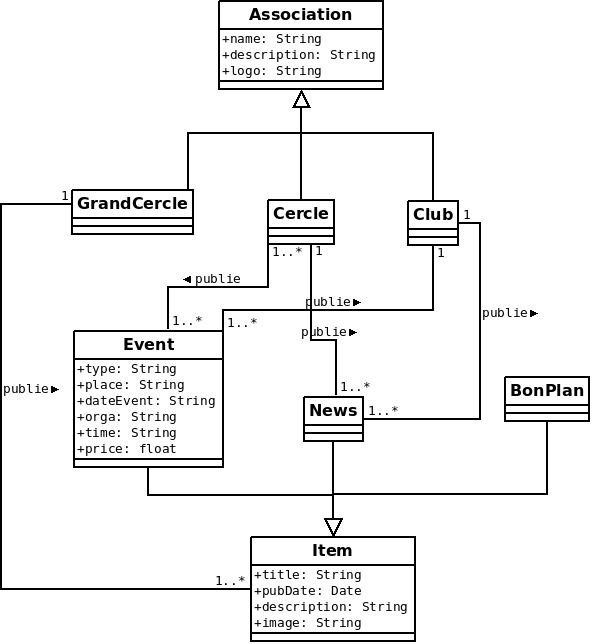
\includegraphics[scale=0.5]{classes.png}
\end{center}
\end{figure}

\section{Présentation technologie}
La technologie android repose sur la dualité entre la langage Java et le langage xml. A chaque affichage correspond un fichier xml qui met en place les différentes fenêtres qui constituent l'écran, appelées des \og layouts \fg, ainsi qu'un fichier Java qui représente ce qu'on appelle une activité, c'est à dire la fenêtre visible à l'écran. La vue offerte à l'utilisateur est mise en place par la méthode setContentView([fichier].xml). Néanmoins, ce fichier xml en paramètre de la méthode mentionnée correspond à une configuration statique de l'affichage. Ainsi, dès que nous avons besoin de modifier dynamiquement une vue, nous le faisons dans le code Java, grâce à l'identifiant de la vue considérée renseigné dans le code xml: c'est ce qui fait la dualité Java/xml. Néanmoins, le placement des différents objets dans les layouts est moins facile en Java que dans un fichier xml, c'est pourquoi nous sommes passé par les fichiers xml dès que cela était possible.\\

Dans la technologie android, c'est un fichier appelé AndroidManifest.xml qui gère les différentes activités de l'application. La première activité lancée est celle contenue dans un label \og intent-filter \fg. Dans notre cas, c'est le fichier GCMLaunching.java qui constitue l'activité de démarrage. Ce dernier fait appel à la méthode \texttt{parseFiles(Context context)} , qui utilise une classe factory pour obtenir une instance d'un SAXParser, nécessaire pour la récupération des données. En effet, l'application réalisée ne peut exister sans que le site du Grand Cercle ne soit tenu à jour. Nous récupérons ainsi toutes les données présentes sur ce site à l'aide de cinq parser, appelés par la méthode \texttt{parseFiles(Context context)}
 sur cinq fichiers xml différents en même temps que l'affichage d'accueil à l'aide de threads.\\

\noindent Plusieurs choses sont ainsi réalisées lors de cette phase:
\begin{itemize}
\item récupération des données sur le site
\item création des listes de clubs, de cercles et de types d'événements, nécessaire pour la gestion des préférences.
\item initialisation de toutes les autres structures de données (listes des données relatives aux événements, aux news, aux bons plans).
\item initialisation de la base de données.
\end{itemize}

\vspace{0.5cm}
\noindent Un des points importants de la récupération de donnée est la présence ou non de connexion internet: 
\begin{itemize}
\item soit une connexion internet est disponible. Dans ce cas on sauvegarde les fichiers xml en provenance du site dans la mémoire et on parse ces données.\\
\item soit aucune connexion n'est possible et dans ce cas, on parse les données qui sont dans la mémoire, sauvegardées lors de connexions antérieures.\\
\end{itemize}

\noindent Lors de la première utilisation de l'application, un message est affiché à l'utilisateur s'il n'est pas connecté à internet pour lui indiquer qu'aucune donnée n'a pu être chargée (mais l'application se lance correctement).
 Lors de l'initialisation de la base de données, aucun filtre n'est appliqué et les données sont récupérées dans leur totalité, l'utilisateur ayant ensuite le choix d'appliquer ou non ces filtres.

Une fois la récupération des données et les initialisations effectuées, l'activité GCM.java est lancée. La différence avec les autres activités est qu'elle étend la classe TabActivity et non Activity. En effet, cette activité permet de construire les onglets de notre application à l'aide d'un objet appelé \texttt{TabHost}. Toutes les vues des différents onglets sont crées dans GCM.java, ce qui permet à l'utilisateur de naviguer rapidement entre les différents onglets.
Au sein de ces onglets, un clic sur les différents boutons lancent d'autres activités à l'aide de \texttt{listeners}.\\

Lors de l'initialisation de la base de données, aucun filtre n'est appliqué et les données sont récupérées dans leur totalité, l'utilisateur ayant ensuite le choix d'appliquer ou non ces filtres.

La base de données est utilisée dans la gestion des préférences, pour choisir les différents filtres ainsi que l'apparence ergonomique. Quatre types de préférences sont proposés à l'utilisateur et pour chaque type, les éléments cochés sont sauvegardés dans la base de données. On effectue alors des tests sur ces données dans les autres activités, notamment pour les couleurs de fond et les filtres sur les données récupérées sur le site du Grand Cercle.\\

Notre application témoigne d'une volonté de simplicité et de rapidité auprès des utilisateurs. Ainsi, la classe \textt{DragableSpace.java} permet de \og slider \fg afin de limiter le nombre d'onglets. le changement de vue n'est réalisé que si l'utilisateur effectue le slide assez rapidement.






\section{Validation}
Les deux applications ont été validées suivant une démarche commune afin d'assurer un niveau de qualité équivalent d'une application à l'autre.

Certains tests ont été réalisés au fur et à mesure du développement des applications, d'autres ont été effectués sur des prototypes fonctionnels et enfin la version finale des deux application a été évaluée par un panel d'utilisateurs potentiels.

\subsection{Tests unitaires}
Chaque module a été testé grâce à des tests unitaires. Majoritairement, ces tests consistent à envoyer en entrée du module un cas de test spécifique, de tracer le module afin de vérifier qu'au cours de l’exécution rien d'anormal ne se produit, et de récupérer en sortie un résultat que l'on compare au résultat attendu. Les tests spécifiques sont pour la plupart des tests dits "boite blanche".

Ces tests sont avant tout des tests techniques qui permettent de s'assurer qu'il n'y a pas d'erreur d'analyse et/ou de programmation.

\subsection{Tests d'intégration et de validation informatique}
Ces tests permettent de tester la cohérence et l'articulation des modules entre eux, de vérifier que les modules communiquent bien entre eux.

Ces tests ont été réalisés de manière similaire aux tests unitaires, à savoir un traçage des opérations effectuées et une comparaison du résultat obtenu avec le résultat attendu.

\subsection{Tests utilisateurs, tests de conformité}
Afin de vérifier la conformité de nos différents prototypes avec les besoins formulés par les utilisateurs, regroupés dans le cahier des charges, nous avons fait appel à un panel d'utilisateurs potentiels disposant de leur propre smartphone sous iOS ou Android, et ce dans le but de confronter ces applications à des utilisateurs habitués aux pratiques sur ces deux systèmes d'exploitation.

Nous avons mis en place des une procédure qui nous a permis de toujours demander à ces utilisateurs potentiels d'effectuer les mêmes manipulations dans l'application et d'observer leur réactions. Pour prendre en compte leurs remarques et ne pas en oublier, nous avons procédé à des enregistrements vidéo de ces tests.

\end{document}
